\section{Modelling Approach}

%The model is formulated as a mixed-integer linear optimization problem with hourly resolution and perfect foresight. It determines the cost-optimal dispatch of the external district heating supply, local heat pumps, heat exchanger flow, and PTES operation while satisfying heat demand and a set of technical operating constraints. Compared to the previous linear formulation, the current model includes binary operating-mode variables for the PTES in order to represent minimum active charging and discharging levels, mutually exclusive operating modes, and a two-hour no-reversal rule between charging and discharging.

To address this limitation, a stylized optimization model is developed that represents economically efficient PTES operation under dynamic pricing signals.

Instead of replicating the current tariff structure, the model introduces a time-dependent marginal cost of heat production that reflects the underlying system economics. This allows the PTES to respond to economically meaningful signals, enabling cost-optimal charging and discharging decisions.

The model is formulated as a linear optimization problem with perfect foresight. It determines the hourly dispatch of all technologies such that total system cost is minimized while satisfying heat demand and technical constraints. In a future version the perfect foresight can be replaced by forecasts, and the optimization can be done using stochastic programming. 

\section{Mathematical Formulation}

The model is formulated as a linear cost-minimization problem over all time steps \( t \in T \), where \(T\) denotes the set of hourly snapshots.

The objective is to minimize total system cost:

\begin{equation}
\min \sum_{t \in T} \left( c^{el}_t g^{el}_t + c^{DH}_t g^{DH}_t \right)
\end{equation}

where:
\begin{itemize}
    \item \(g^{el}_t\) denotes electricity consumption from the electricity market [MW],
    \item \(g^{DH}_t\) denotes heat supplied by the external district heating system [MW],
    \item \(c^{el}_t\) is the electricity price [DKK/MWh],
    \item \(c^{DH}_t\) is the marginal cost of external heat production [DKK/MWh].
\end{itemize}

The optimization is subject to energy balance constraints, technology-specific conversion relationships, capacity limits, and storage dynamics.

\subsection{Energy Balances}

\subsubsection*{Electricity balance} 

Electricity consumption supplies the heat pumps:

\begin{equation}
g^{el}_{t} = p^{c2}_{t} + p^{gw}_{t}
\end{equation}

where \(p^{c2}_{t}\) and \(p^{gw}_{t}\) denote the electrical input of the City 2 heat pump and the groundwater heat pump, respectively [MW].

\subsubsection*{Main district heating system} 

Heat supplied by the external system is either transferred to the local system or used to charge the PTES:

\begin{equation}
g^{DH}_{t} = f^{HX}_{t} + p^{ch}_{t}
\end{equation}

where \(f^{HX}_{t}\) denotes the heat flow through the heat exchanger [MW] and \(p^{ch}_{t}\) is the PTES charging power [MW].

\subsubsection*{Høje Taastrup district heating system}

The local heat demand must be met at all times:

\begin{equation}
f^{HX}_{t} + q^{c2}_{t} + q^{gw}_{t} + p^{dis}_{t} = d_t
\end{equation}

where:
\begin{itemize}
    \item \(q^{c2}_{t}\), \(q^{gw}_{t}\) denote heat output from the City 2 and groundwater heat pumps [MW],
    \item \(p^{dis}_{t}\) is the PTES discharging power [MW],
    \item \(d_t\) is the exogenous heat demand [MW].
\end{itemize}

\subsection{Technology Constraints}

Heat pump operation is defined by their coefficient of performance (COP):

\begin{align}
q^{c2}_{t} &= COP^{c2}_{t} \cdot p^{c2}_{t} \\
q^{gw}_{t} &= COP^{gw}_{t} \cdot p^{gw}_{t}
\end{align}

where \(COP^{c2}_{t}\) and \(COP^{gw}_{t}\) denote the time-dependent coefficients of performance of the City 2 and groundwater heat pump, respectively.

The electrical input of both heat pumps is limited by their installed capacities:

\begin{align}
0 \le p^{c2}_{t} &\le \bar{p}^{c2} \\
0 \le p^{gw}_{t} &\le \bar{p}^{gw}
\end{align}

where \(\bar{p}^{c2}\) and \(\bar{p}^{gw}\) denote the installed electrical capacities of the City 2 and groundwater heat pump, respectively [MW].

The heat transfer through the heat exchanger is limited by:

\begin{equation}
0 \le f^{HX}_{t} \le \bar{f}^{HX}
\end{equation}

where \(\bar{f}^{HX}\) denotes the maximum heat transfer capacity of the heat exchanger [MW].

\subsection{PTES Dynamics}

The PTES state of charge evolves according to:

\begin{equation}
e_t = (1-\lambda)e_{t-1} + p^{ch}_{t} - p^{dis}_{t}
\end{equation}

where:
\begin{itemize}
    \item \(e_t\) denotes the stored thermal energy [MWh],
    \item \(\lambda\) represents standing losses [-].
\end{itemize}

The storage level and charging/discharging power are bounded by:

\begin{align}
0 \le e_t &\le \bar{e} \\
0 \le p^{ch}_{t} &\le \bar{p}^{ch} \\
0 \le p^{dis}_{t} &\le \bar{p}^{dis}
\end{align}

where:
\begin{itemize}
    \item \(\bar{e}\) is the maximum PTES energy capacity [MWh],
    \item \(\bar{p}^{ch}\) is the maximum charging power [MW],
    \item \(\bar{p}^{dis}\) is the maximum discharging power [MW].
\end{itemize}

The storage is initialized with a given state of charge:

\begin{equation}
e_0 = e^{init}
\end{equation}

where \(e^{init}\) denotes the initial energy content of the PTES [MWh].

To ensure cyclic operation over the optimization horizon, the final state of charge is constrained to equal the initial state:

\begin{equation}
e_{|T|} = e_0
\end{equation}

All decision variables are restricted to be non-negative.

\section{Marginal Cost of External Heat Production}

A central element of the model is the representation of the external district heating system through a time-varying marginal cost of heat production.

The external system is approximated by a stylized combined heat and power (CHP) unit. The marginal cost of heat production is derived using an opportunity-cost formulation that captures the joint production of heat and electricity.

For all \( t \in T \), the marginal heat production cost is defined as:

\begin{equation}
MC^{heat}_{t}
=
\frac{c_f}{\eta_{th}}
-
c^{el}_{t}\frac{\eta_{el}}{\eta_{th}}
\end{equation}

where:
\begin{itemize}
    \item \(c_f\) is the fuel cost [DKK/MWh$_{fuel}$],
    \item \(\eta_{th}\), \(\eta_{el}\) are the thermal and electrical efficiencies [-],
    \item \(c^{el}_{t}\) is the electricity price [DKK/MWh].
\end{itemize}

The first term represents the fuel cost per unit of heat output, while the second term reflects the electricity revenue associated with CHP production. Consequently, the marginal cost of heat production decreases with increasing electricity prices.

This formulation introduces a direct coupling between the electricity market and heat production costs. Periods with high electricity prices correspond to low marginal heat costs, while low electricity prices result in higher effective heat production costs.

The marginal cost is bounded from below to avoid non-physical values:

\begin{equation}
c^{DH}_{t} = \max(0, MC^{heat}_{t})
\end{equation}

The following parameter values are assumed:

\begin{equation}
c_f = 180 \ \text{DKK/MWh}_{fuel}, \quad
\eta_{th} = 0.45, \quad
\eta_{el} = 0.40
\end{equation}

\section{Results}

\subsection{Current Operation}

To assess the current utilisation of the PTES, historical operational data for the year 2024 is analysed.

\begin{figure}[H]
    \centering
    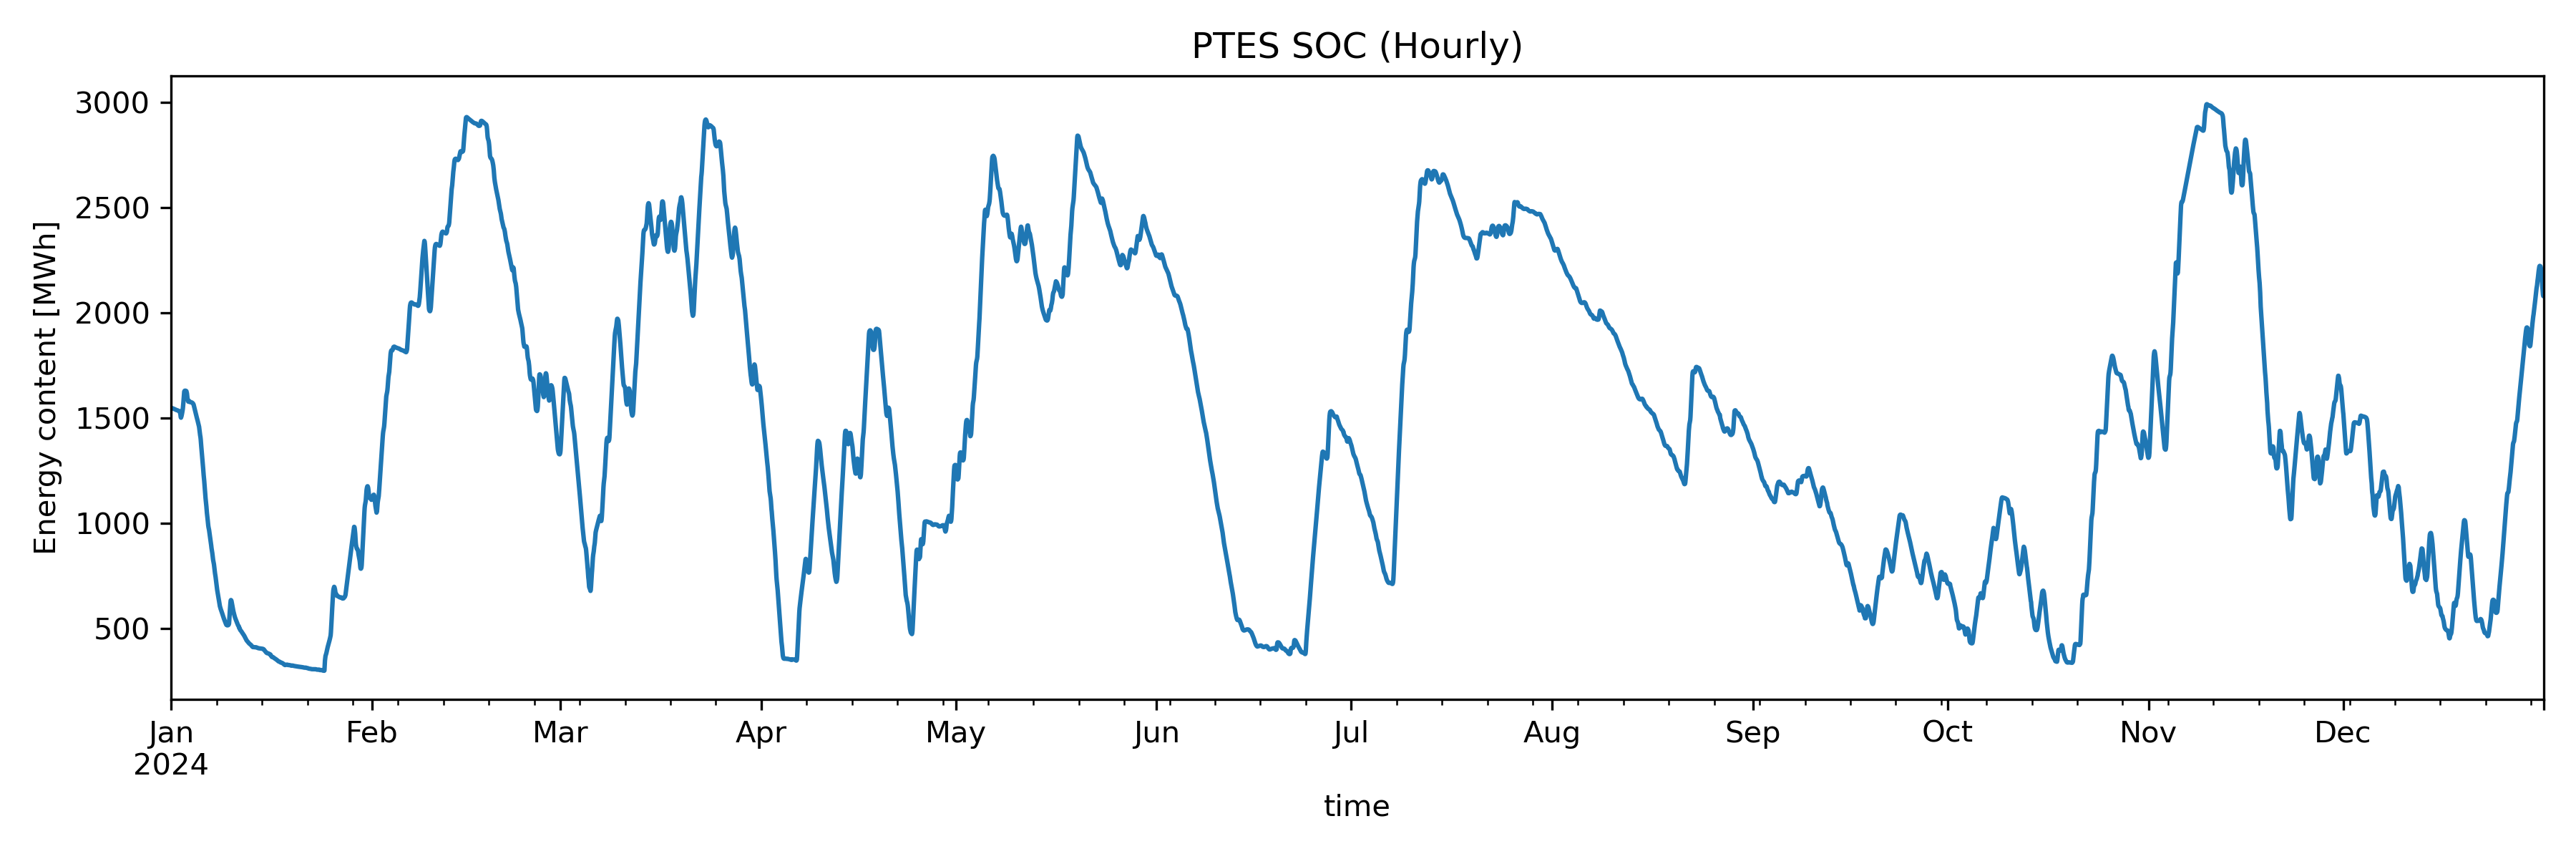
\includegraphics[width=0.9\linewidth]{figures/paper_figure/ptes_soc_hourly.png}
    \caption{State of charge of the PTES based on measured data for 2024}
    \label{fig:ptes_real_soc}
\end{figure}

The observed operation corresponds to approximately 10 full equivalent cycles per year, defined as the ratio of total discharged energy to usable storage capacity.

This is significantly below the intended operational range of approximately 25--30 cycles per year, indicating that the storage is not utilised to its full technical potential.

\subsection{Optimized Operation}

Using the digital twin model and given the introduced marginal cost formulation, the model exhibits economically driven charging and discharging behaviour. Figure~\ref{fig:ptes_optimized} shows the resulting state of charge of the PTES under optimal operations. 

\begin{figure}[H]
    \centering
    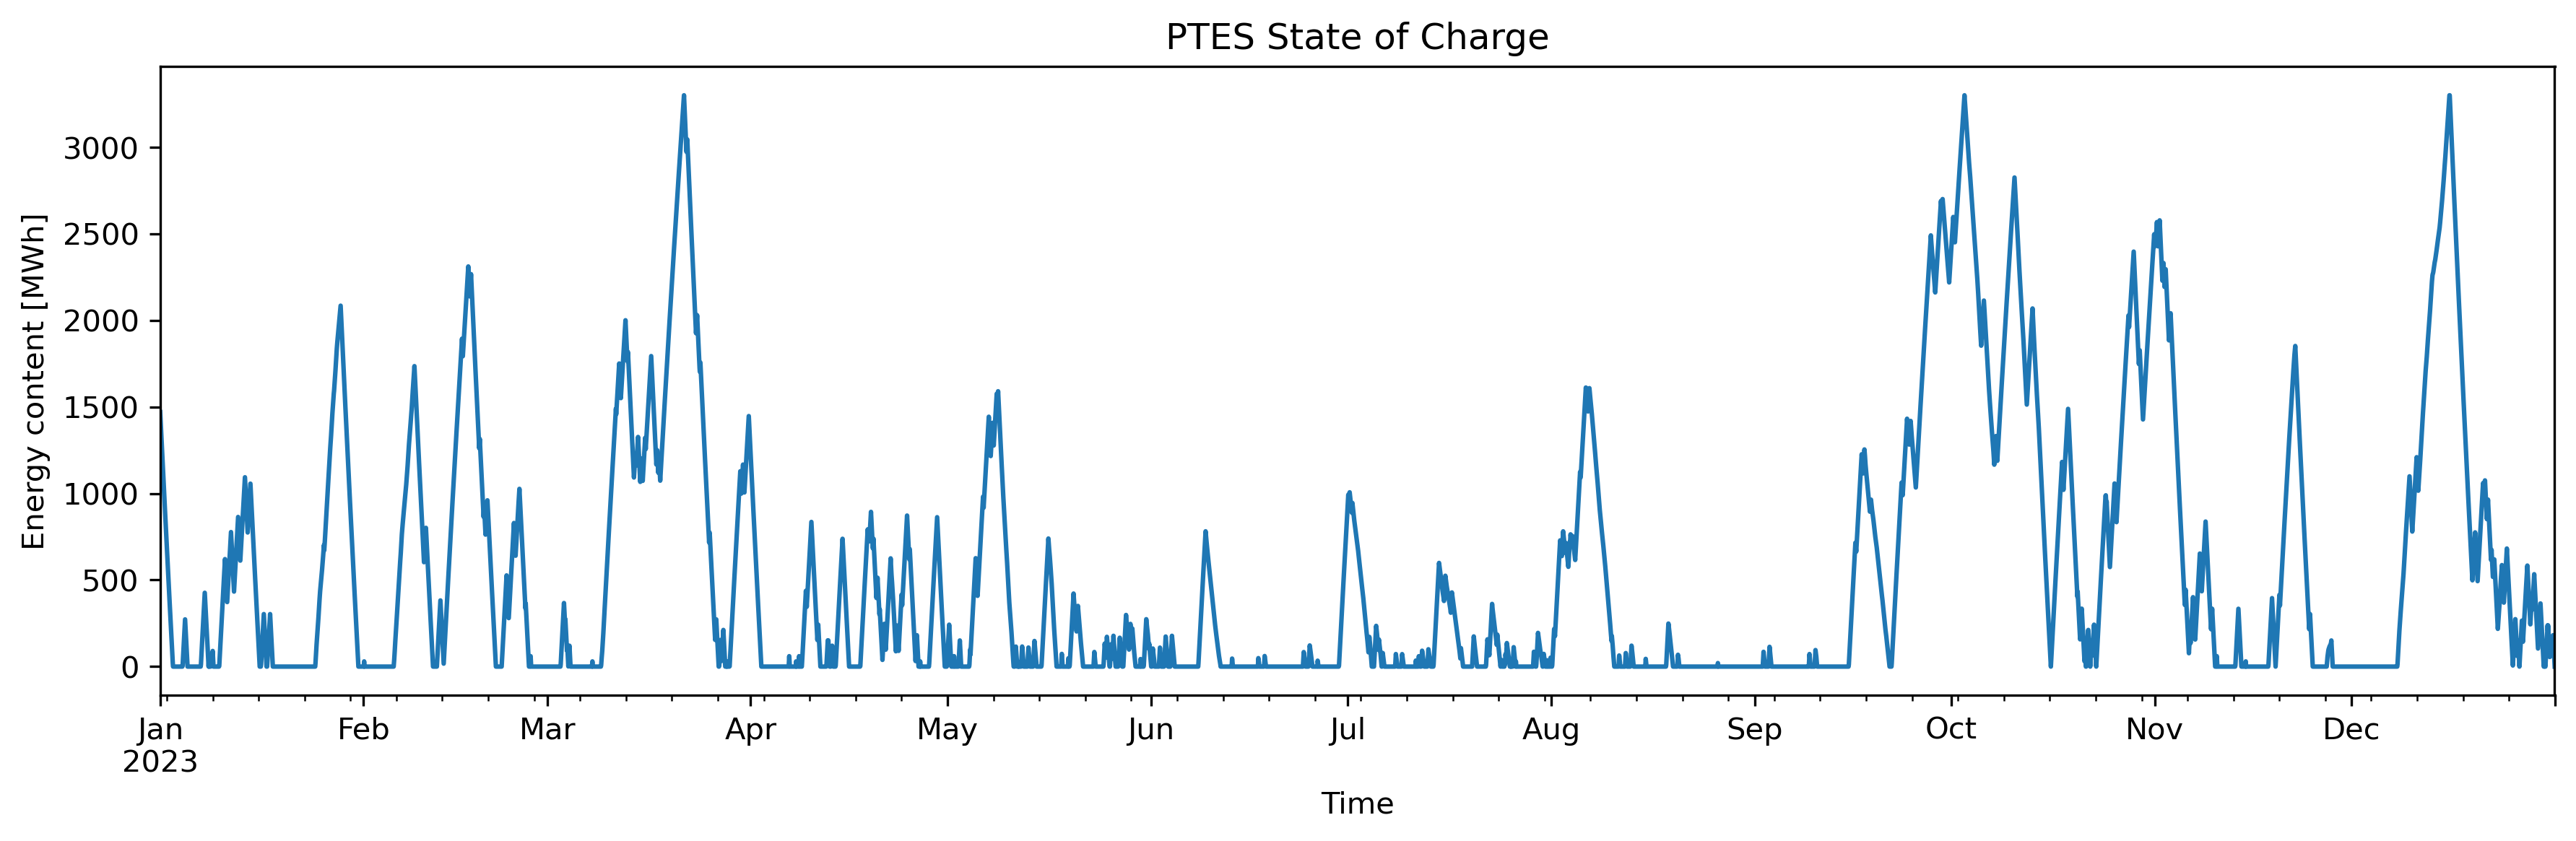
\includegraphics[width=0.9\linewidth]{figures/paper_figure/ptes_soc.png}
    \caption{Optimised PTES state of charge under dynamic pricing}
    \label{fig:ptes_optimized}
\end{figure}

The optimised operation results in approximately 33 full equivalent cycles per year, which is close to the intended operational range.

Although the storage does not always reach its maximum capacity of 3300 MWh, the results demonstrate a substantial increase in utilisation compared to historical operation and highlight the flexibility potential of the PTES under dynamic pricing conditions.

\subsection{Heat Pump Operation}

\begin{figure}[H]
    \centering
    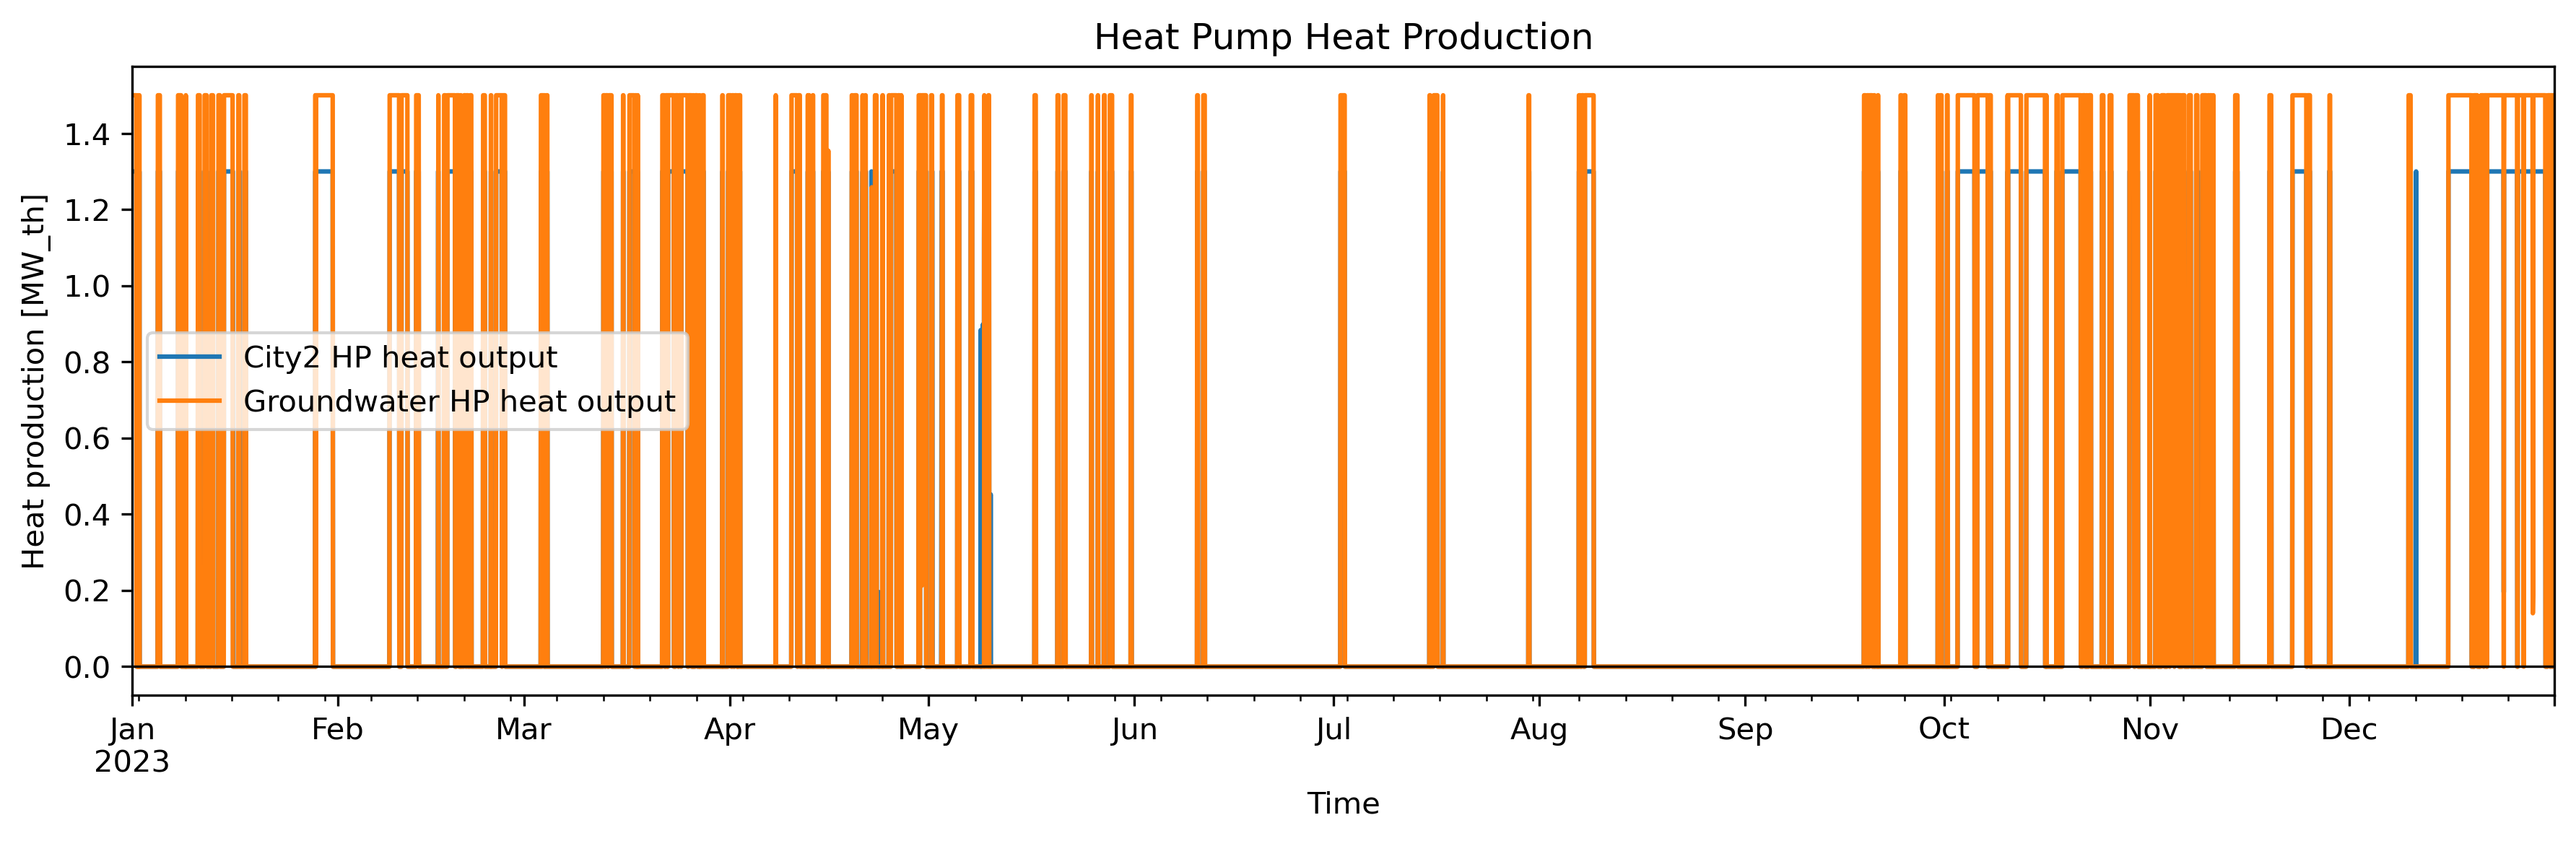
\includegraphics[width=0.9\linewidth]{figures/paper_figure/heat_pump_production.png}
    \caption{Heat generation of the modelled heat pumps}
    \label{fig:heat_pumps}
\end{figure}

The model includes two heat pump technologies, both of which contribute to heat production under the current parameterisation. Their operation is determined endogenously by the optimisation and reflects the interaction between electricity prices, coefficient of performance, and system constraints.

Overall, the contribution of heat pumps remains relatively small compared to total demand. According to HT DH, approximately 20\% of the heat demand can be covered by local production. This share is not yet reproduced in the current model, suggesting that additional components or improved parameterisation are required.

\section{Discussion}

\section{Conclusion}